\documentclass[conference]{IEEEtran}
\IEEEoverridecommandlockouts
% The preceding line is only needed to identify funding in the first footnote. If that is unneeded, please comment it out.
\usepackage{cite}
\usepackage{amsmath,amssymb,amsfonts}
\usepackage{algorithmic}
\usepackage{graphicx}
\usepackage{textcomp}
\usepackage{xcolor}
\usepackage{placeins}
\def\BibTeX{{\rm B\kern-.05em{\sc i\kern-.025em b}\kern-.08em
    T\kern-.1667em\lower.7ex\hbox{E}\kern-.125emX}}
\begin{document}

\title{Rangefinder-Disciplined Visual Object Detection}

\author{
	\IEEEauthorblockN{Raj Anadkat}
	\IEEEauthorblockA{raj618@seas.upenn.edu}
\and
	\IEEEauthorblockN{Jonathan Lee}
	\IEEEauthorblockA{jonlee27@seas.upenn.edu}
\and
	\IEEEauthorblockN{Jonathan Schoeffling}
	\IEEEauthorblockA{jschoeff@seas.upenn.edu}
\and
	\IEEEauthorblockN{Hanli Zhang}
	\IEEEauthorblockA{hanlizh@seas.upenn.edu}
}

\maketitle

\begin{abstract}
The lidar used on the F1TENTH platform is expensive, which limits the size of
the classes and programs that use it. By fusing data from high azimuth accuracy
/ low range accuracy sensors with data from low azimuth accuracy / high range
accuracy accuracy sensors, a more useful combined estimate of both azimuth and
range may be achieved.
\end{abstract}

\begin{IEEEkeywords}
F1TENTH, autonomous driving, MiDaS, time-of-flight, rangefinder, lidar, sensor
fusion
\end{IEEEkeywords}

\section{What is the problem?}
To function as an autonomous vehicle, the F1TENTH platform must be able to
determine the location of objects in its environment, with a reasonable degree
of accuracy in both azimuth and range. While the lidars currently used are more
than adequate for this task, they are also expensive, making up a significant
percentage of the overall cost of the platform.


\section{Why is it important?}
As an educational program, material cost can be a significant factor for the
F1TENTH program. If a sufficiently accurate method of object detection using
less expensive components can be developed, the F1TENTH platform would become
more accessible. A greater number of vehicles could be produced for the same
cost, allowing for larger course sizes or participation by institutions that
are more resource-constrained.


\section{Why is it hard?}
A lidar is precision device, usually with moving parts, making it more
expensive to produce. Less expensive components may achieve comparable accuracy
to a lidar in some dimensions, but generally cannot do so across all required
dimensions. If the outputs of inexpensive sensors that are accurate in a subset
of the required dimensions can be combined, significant cost savings may be
realized.

\section{What have others tried to do?}
Stereo Camera

MiDaS \cite{midas}


\section{What you will do? How long will it take?}
\subsection{Scope of Work}
The aim of the project is to use sensor fusion to combine the strengths of
MiDaS and low-cost laser rangefinders.

As a camera-driven algorithm, MiDaS can produce outputs with high accuracy in
azimuth and elevation, but only low-fidelity depth estimates. Determining
\textit{relative} depth appears to be fairly reliable (the default output is a
normalized range of depth values), but accuracy can suffer when making the
association to absolute distance measurements. While this can be mitigated by
training the model for a specific environment, such an approach is unlikely to
generalize well, limiting its utility.

By contrast, an array of rangefinders has excellent accuracy in depth, but can
only provide azimuth information in a fixed angle increments with a fairly wide
field of view. Consequently, such an approach is, on its own, unsuitable for
fine measurements in azimuth. The VL53L4CX time-of-flight sensor selected for
this project provides a histogram of the intensity of each reflection within
its 18° field of view and across its 6m range.

\begin{figure}
\centering
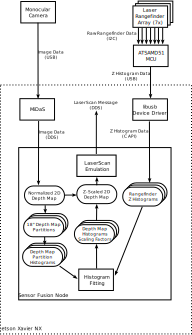
\includegraphics[scale=0.31]{block-diagram.png}
\caption{Block diagram for the sensor system}
\label{fig:block-diagram}
\end{figure}

\FloatBarrier

The histogram output of the VL53L4CX provides a very useful input for the
sensor fusion implementation. By overlapping the rangefinders' fields of view
with the corresponding sections of the MiDaS depth map, accurate depth data can
be determined for the corresponding image sections. By taking an intensity
histogram of the depth map, a direct comparison of estimated and measured range
becomes possible. The sensor fusion algorithm can correlate the intensity peaks
in both histograms, and produce a scaling factor for each section of the
normalized depth map through simple linear regression. The architecture and
data flows are illustrated in Figure \ref{fig:block-diagram}.

This approach has the potential to provide reasonable accuracy in both range
and azimuth using relatively inexpensive components. If successful, the sensor
fusion approach would provide adequate capabilities at a fraction of the cost
of the current sensor. Active measurement using the time-of-flight rangefinders
should allow the implementation to generalize to other environments.


\subsection{Project Schedule and Risks}

\FloatBarrier

\begin{figure}
\centering
\includegraphics[scale=0.18]{schedule.png}
\caption{Project schedule}
\label{fig:schedule}
\end{figure}

The project schedule is illustrated in Figure \ref{fig:schedule}. The proposed
timeline is aggressive, but feasible with a four-person team. Critical-path
items include material orders and configuring the MiDaS model to run on the
Jetson in order to provide initial sample data for the sensor fusion
implementation.

Potential risks include the following:
\begin{itemize}
\item If the computational requirements of the MiDaS model and other nodes of
the F1TENTH stack exceed the capabilities of the Jetson, integration of a
dedicated processor may be required, increasing project scope.

\item If the update rate of the sensor sources is substantially lower than that
of the lidar, the maximum speed of the vehicle may be limited.

\item If material is delayed, firmware development time may be impacted.
\end{itemize}

\FloatBarrier

\section{How you will measure success?}
At a proof-of-concept level, success of the implementation can be assessed
by directly measuring distances to obstructions in a known environment, and
comparing the output of the rangefinder-disciplined MiDaS depth map to those
measurements. The full accuracy of the lidar is not necessary in most
situations, so a reasonable approximation can be considered a success.

From a practical perspective, a successful implementation would be capable of
replacing the lidar on the vehicle. Sufficient accuracy may be demonstrated if
the platform can execute a follow-the-gap algorithm with sensor inputs coming
from the augmented depth map.


\begin{thebibliography}{00}
\bibitem{midas} Ranftl et. al., Towards Robust Monocular Depth Estimation:
Mixing Datasets for Zero-shot Cross-dataset Transfer, TPAMI 2022
\end{thebibliography}

\end{document}
